\documentclass[letterpaper,12pt]{article}
\usepackage{array}
\usepackage{threeparttable}
\usepackage{geometry}
\geometry{letterpaper,tmargin=1in,bmargin=1in,lmargin=1.25in,rmargin=1.25in}
\usepackage{fancyhdr,lastpage}
\pagestyle{fancy}
\lhead{}
\chead{}
\rhead{}
\lfoot{}
\cfoot{}
\rfoot{\footnotesize\textsl{Page \thepage\ of \pageref{LastPage}}}
\renewcommand\headrulewidth{0pt}
\renewcommand\footrulewidth{0pt}
\usepackage[format=hang,font=normalsize,labelfont=bf]{caption}
\usepackage{listings}
\lstset{frame=single,
  language=Python,
  showstringspaces=false,
  columns=flexible,
  basicstyle={\small\ttfamily},
  numbers=none,
  breaklines=true,
  breakatwhitespace=true
  tabsize=3
}
\usepackage{amsmath}
\usepackage{amssymb}
\usepackage{amsthm}
\usepackage{harvard}
\usepackage{setspace}
\usepackage{float,color}
\usepackage[pdftex]{graphicx}
\usepackage{hyperref}
\hypersetup{colorlinks,linkcolor=red,urlcolor=blue}
\theoremstyle{definition}
\newtheorem{theorem}{Theorem}
\newtheorem{acknowledgement}[theorem]{Acknowledgement}
\newtheorem{algorithm}[theorem]{Algorithm}
\newtheorem{axiom}[theorem]{Axiom}
\newtheorem{case}[theorem]{Case}
\newtheorem{claim}[theorem]{Claim}
\newtheorem{conclusion}[theorem]{Conclusion}
\newtheorem{condition}[theorem]{Condition}
\newtheorem{conjecture}[theorem]{Conjecture}
\newtheorem{corollary}[theorem]{Corollary}
\newtheorem{criterion}[theorem]{Criterion}
\newtheorem{definition}[theorem]{Definition}
\newtheorem{derivation}{Derivation} % Number derivations on their own
\newtheorem{example}[theorem]{Example}
\newtheorem{exercise}[theorem]{Exercise}
\newtheorem{lemma}[theorem]{Lemma}
\newtheorem{notation}[theorem]{Notation}
\newtheorem{problem}[theorem]{Problem}
\newtheorem{proposition}{Proposition} % Number propositions on their own
\newtheorem{remark}[theorem]{Remark}
\newtheorem{solution}[theorem]{Solution}
\newtheorem{summary}[theorem]{Summary}
%\numberwithin{equation}{section}
\bibliographystyle{aer}
%\newcommand\ve{\varepsilon}
%\newcommand\boldline{\arrayrulewidth{1pt}\hline}


\begin{document}

\begin{flushleft}
  \textbf{\large{Problem Set \#[2]}} \\
  MACS 40000, Dr. Evans \\
  Fiona Fan
\end{flushleft}

\vspace{5mm}

\noindent\textbf{Problem 1}
\\ \textbf{Part (a).} The first period consumption, $c_1$ is negative, most possibly resulted from a excessively big $b_1$.
\\ \textbf{Part (b).} No constraint is violated.
\\ \textbf{Part (c).} No constraint is violated.\\




\noindent\textbf{Problem 2} \\
\textbf{Part (a).} See the first column of Table \ref{table1} for results. The computations took 0.0028s and 0.0020s respectively.

\textbf{Part (b).} Please see Figure \ref{Fig1}. 

\textbf{Part (c).} \par See the second column of Table \ref{table1} for results. All metrics increase except for $\bar{r}$. As $\beta$ increases, the agents become more patient towards future rewards, discounting them less. This would lead them to save more as they value the savings in the future comparatively more as they become more patient. \par $\bar{K}$ increases because it's the aggregate of all savings. $\bar{L}$ remains unchanged because it's exogenous. The increase in $\bar{K}$ will result in increase in both $\bar{r}$ and $\bar{w}$ because other parameters like A, $\alpha$ and $\delta$ remain unchanged. \par The consumptions increase because the income effect overshadows the substitution effect, as households' wages increase.\\ 


\noindent\textbf{Problem 3}\\
\textbf{Part (a).} Please see Figure \ref{fig2}, Figure \ref{fig3} and Figure \ref{fig4} for $\{{K_t}_{t=1}^{T+5}\}$, $\{{w_t}_{t=1}^{T+5}\}$ and $\{{r_t}_{t=1}^{T+5}\}$ respectively.


\noindent\textbf{Part (b).} In period 3, the economy first gets to within 0.00001 of the steady state. After period 11, the economy is never again father than 0.00001 away from the steady state.

\begin{table}[ht]
	\captionsetup{width=6.0in}
	\caption{Steady State Results for Varying $\beta$s} % title of Table
	\centering 
	\begin{tabular}{c c c} % centered columns (4 columns)
		\hline\hline %inserts double horizontal lines
		Output & $\beta=0.195$ & $\beta=0.55$ \\ [0.5ex] % inserts table
		%heading
		\hline % inserts single horizontal line
		$\bar{b_2}$ & 0.019 & 0.028  \\ % inserting body of the table
		$\bar{b_3}$ & 0.058 & 0.077  \\
		$\bar{K}$ & 0.078 & 0.105 \\
		$\bar{L}$ & 2.2 & 2.2 \\
		$\bar{w}$ & 0.202 & 0.224 \\
		$\bar{r}$ & 2.433 & 1.886 \\ 
		$\bar{c_1}$ & 0.182 & 0.196 \\ 
		$\bar{c_2}$ & 0.210 & 0.229 \\ 
		$\bar{c_3}$ & 0.241 & 0.267 \\ [1ex] % [1ex] adds vertical space
		\hline %inserts single line
	\end{tabular}
	\label{table1} % is used to refer this table in the text
\end{table}

\begin{figure}[htb]\centering
	\captionsetup{width=4.0in}
	\caption{\textbf{Steady-State Distribution of Consumption and Savings by Age}}
	\label{Fig1}
	\fbox{\resizebox{4.0in}{3.0in}{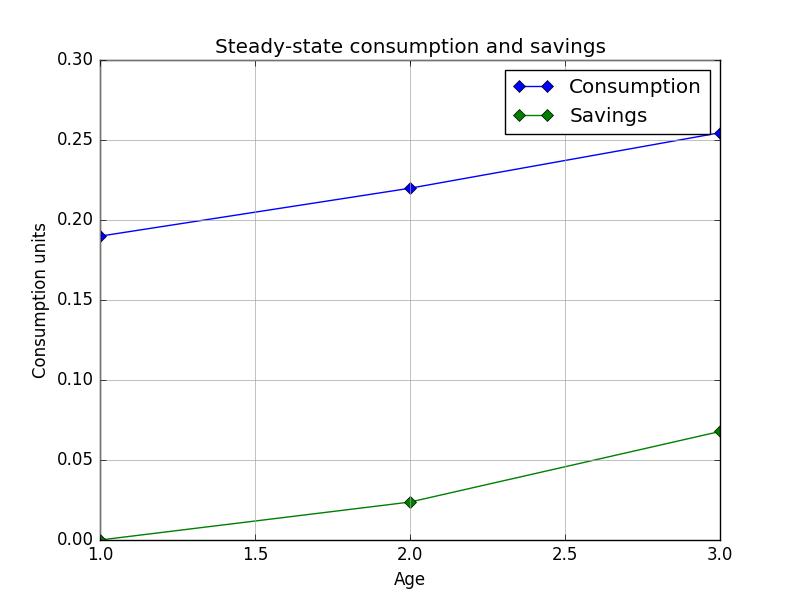
\includegraphics{figure_0.png}}}
\end{figure}

\begin{figure}[htb]\centering
	\captionsetup{width=4.0in}
	\caption{\textbf{$\{{K_t}_{t=1}^{T+5}\}$}} \label{fig2}
	\fbox{\resizebox{4.0in}{3.0in}{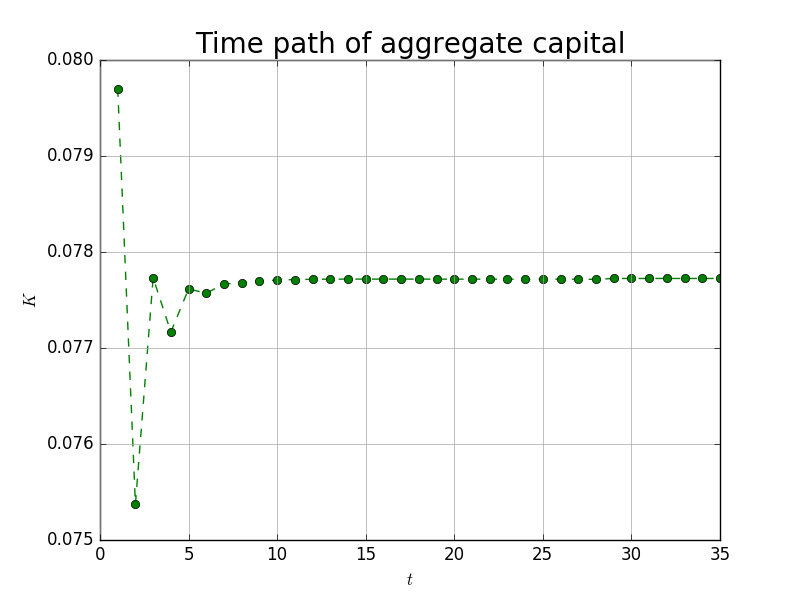
\includegraphics{figure_2.png}}}
\end{figure}

\begin{figure}[htb]\centering
	\captionsetup{width=4.0in}
	\caption{\textbf{$\{{w_t}_{t=1}^{T+5}\}$}}
	\label{fig3}
	\fbox{\resizebox{4.0in}{3.0in}{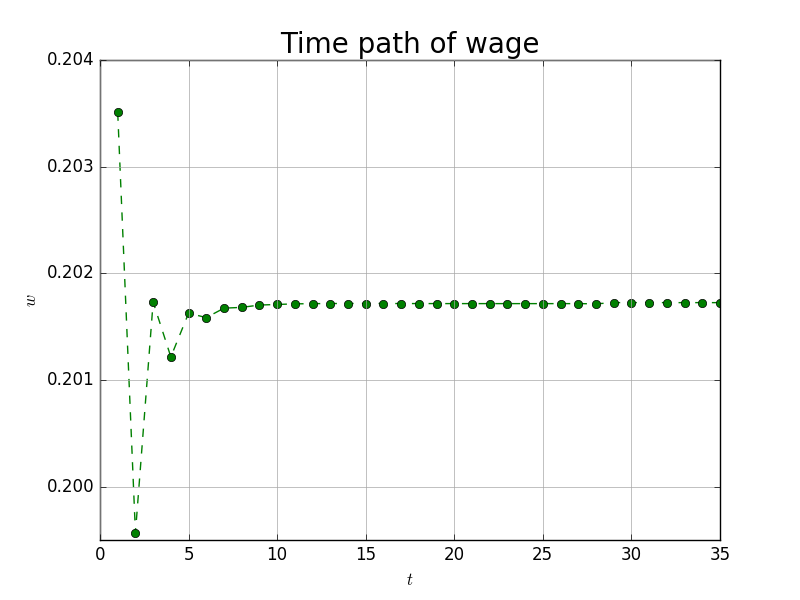
\includegraphics{figure_3.png}}}
\end{figure}

\begin{figure}[htb]\centering
	\captionsetup{width=4.0in}
	\caption{\textbf{$\{{r_t}_{t=1}^{T+5}\}$}}
	\label{fig4}
	\fbox{\resizebox{4.0in}{3.0in}{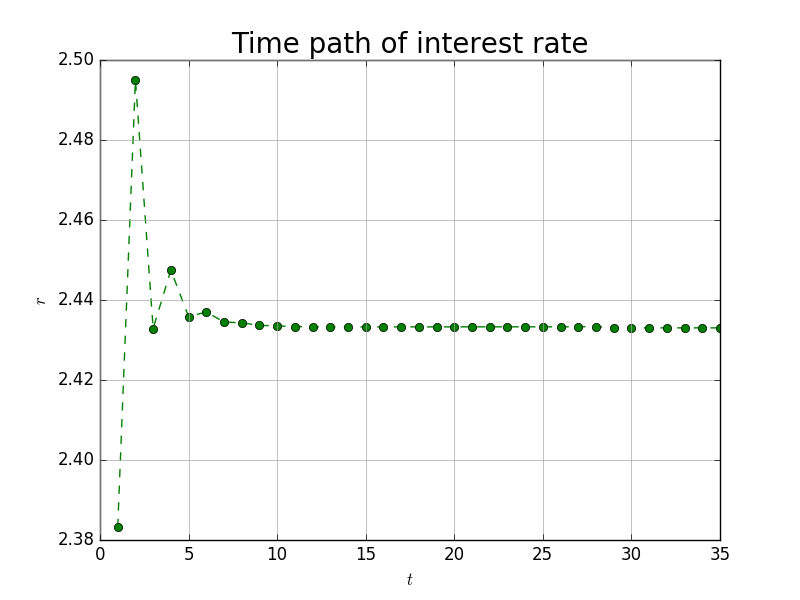
\includegraphics{figure_4.png}}}
\end{figure}


\end{document}

